\documentclass[aspectratio=169,10pt]{beamer}

\usepackage[T1]{fontenc}
\usepackage{lmodern}
\usepackage{graphicx}
\usepackage{booktabs}
\usepackage{array}
\usepackage{hyperref}
\usepackage{xcolor}

\definecolor{Navy}{HTML}{111827}
\definecolor{Ink}{HTML}{E5E7EB}
\definecolor{Muted}{HTML}{9CA3AF}
\definecolor{Cyan}{HTML}{22D3EE}
\definecolor{Pink}{HTML}{F472B6}
\definecolor{Green}{HTML}{34D399}
\definecolor{Amber}{HTML}{FBBF24}

\setbeamercolor{normal text}{fg=Ink,bg=Navy}
\setbeamercolor{frametitle}{fg=white,bg=Navy}
\setbeamercolor{structure}{fg=Cyan}
\setbeamercolor{alerted text}{fg=Pink}
\setbeamercolor{footline}{fg=Muted,bg=Navy}
\setbeamerfont{frametitle}{size=\Large,series=\bfseries}
\setbeamerfont{normal text}{size=\small}
\setbeamertemplate{navigation symbols}{}
\setbeamertemplate{itemize item}{\color{Cyan}\raise0.15ex\hbox{\scriptsize$\blacktriangleright$}}
\setbeamertemplate{itemize subitem}{\color{Pink}\raise0.15ex\hbox{\tiny$\bullet$}}
\setbeamertemplate{footline}{%
  \leavevmode\hbox{%
  \begin{beamercolorbox}[wd=.84\paperwidth,ht=2.8ex,dp=1.2ex,leftskip=.45cm]{footline}%
    Bao et al., ICCV 2017 \quad arXiv:1703.10155
  \end{beamercolorbox}%
  \begin{beamercolorbox}[wd=.16\paperwidth,ht=2.8ex,dp=1.2ex,rightskip=.45cm plus1fil]{footline}%
    \insertframenumber/5
  \end{beamercolorbox}}%
}
\setbeamersize{text margin left=0.55cm,text margin right=0.55cm}

% Replace this placeholder with the repository used for your reproduction.
\newcommand{\RepoURL}{https://github.com/sivajeetsabdakar/cvae-gan-pytorch-reproduction}
\newcommand{\pending}{\textcolor{Amber}{\textbf{Pending}}}
\newcommand{\source}[1]{\par\vspace{0.15em}{\tiny\color{Muted}#1}}

\begin{document}

% Slide 1
\begin{frame}{Paper overview}
\begin{columns}[T,onlytextwidth]
  \begin{column}{0.57\textwidth}
    {\Large\bfseries CVAE-GAN: Fine-Grained Image Generation through Asymmetric Training}\par
    \vspace{0.35em}
    {\color{Cyan}Jianmin Bao, Dong Chen, Fang Wen, Houqiang Li, Gang Hua}\par
    {\footnotesize ICCV 2017, Venice, Italy \quad DOI: 10.1109/ICCV.2017.299}
    \vspace{0.6em}
    \footnotesize
    \begin{itemize}\setlength\itemsep{0.28em}
      \item \textbf{Problem:} conditional generators struggle to produce images that are realistic, diverse, and faithful to a fine-grained class.
      \item \textbf{Motivation:} VAE outputs tend to blur; GAN training can suffer from unstable gradients and mode collapse.
      \item \textbf{Main contribution:} a conditional VAE-GAN with asymmetric objectives, mean feature matching, and pairwise reconstruction constraints.
      \item \textbf{Project code:} \href{\RepoURL}{\textcolor{Cyan}{\RepoURL}}
    \end{itemize}
  \end{column}
  \begin{column}{0.40\textwidth}
    \vspace{0.25em}
    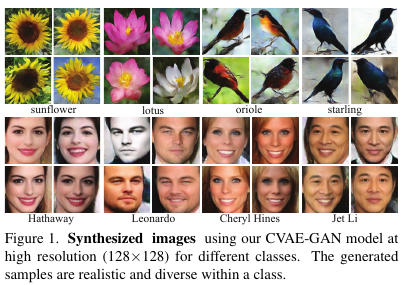
\includegraphics[width=\linewidth]{assets/paper_samples.png}
    \source{Paper Figure 1: 128$\times$128 class-conditioned samples.}
  \end{column}
\end{columns}
\end{frame}

% Slide 2
\begin{frame}{Methodology}
\begin{columns}[T,onlytextwidth]
  \begin{column}{0.47\textwidth}
    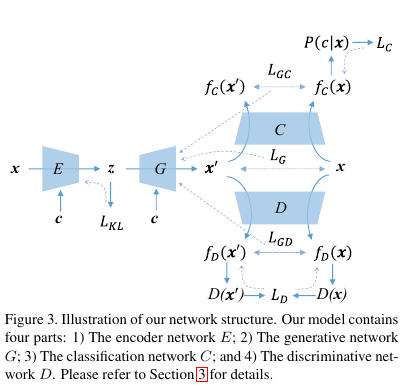
\includegraphics[width=\linewidth,height=0.52\textheight,keepaspectratio]{assets/architecture.png}
    \source{Paper Figure 3: encoder $E$, generator $G$, classifier $C$, discriminator $D$.}
  \end{column}
  \begin{column}{0.50\textwidth}
    \begin{itemize}\setlength\itemsep{0.38em}
      \item \textbf{Workflow:} $E(x,c)$ infers latent $z$; $G(z,c)$ reconstructs or samples $x'$; $C$ preserves class identity; $D$ enforces realism.
      \item \textbf{Datasets:} FaceScrub, Oxford 102 Flowers, and CUB-200 birds.
      \item \textbf{Generator objective:} combine pixel reconstruction, discriminator-feature matching, and classifier-feature matching.
      \item \textbf{Asymmetric training:} $C$ and $D$ use cross-entropy, while $G$ matches feature means with an $\ell_2$ objective.
      \item \textbf{Key settings:} $128\times128$ images, 256-D latent code, batch normalization, $\lambda_1=3$, $\lambda_2=1$, $\lambda_3=\lambda_4=10^{-3}$.
    \end{itemize}
  \end{column}
\end{columns}
\end{frame}

% Slide 3
\begin{frame}{Reproduction and implementation}
\begin{columns}[T,onlytextwidth]
  \begin{column}{0.45\textwidth}
    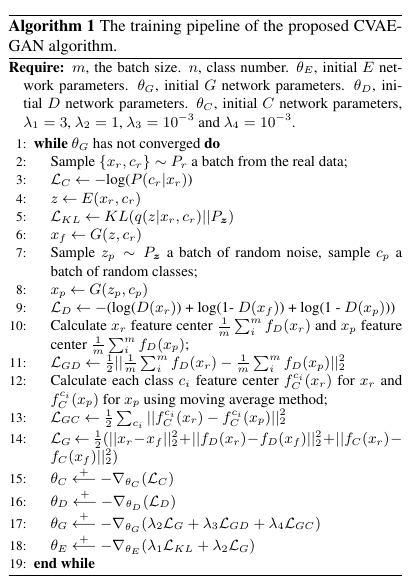
\includegraphics[width=\linewidth,height=0.73\textheight,keepaspectratio]{assets/algorithm.png}
    \source{Paper Algorithm 1: alternating updates for $C$, $D$, $G$, and $E$.}
  \end{column}
  \begin{column}{0.52\textwidth}
    \footnotesize
    \begin{itemize}\setlength\itemsep{0.28em}
      \item \textbf{Original toolchain:} Torch; GoogLeNet encoder, six-layer deconvolutional generator, DCGAN discriminator, AlexNet classifier.
      \item \textbf{Dataset preparation:} align FaceScrub faces from five landmarks; crop Oxford Flowers using masks; retain original CUB-200 images; resize inputs to $128\times128$.
      \item \textbf{Implementation approach:} alternate network updates exactly as Algorithm 1 and use moving averages for class-specific feature centers.
      \item \textbf{Experimental setup:} train all networks from scratch; sample $z\sim\mathcal{N}(0,I)$ for category-conditioned testing.
      \item \textbf{Implementation status:} PyTorch code, shape/loss tests, checkpointing, sampling, and a one-step CPU smoke run are verified. Paper-scale training remains \pending.
    \end{itemize}
  \end{column}
\end{columns}
\end{frame}

% Slide 4
\begin{frame}{Results and comparison}
\begin{columns}[T,onlytextwidth]
  \begin{column}{0.54\textwidth}
    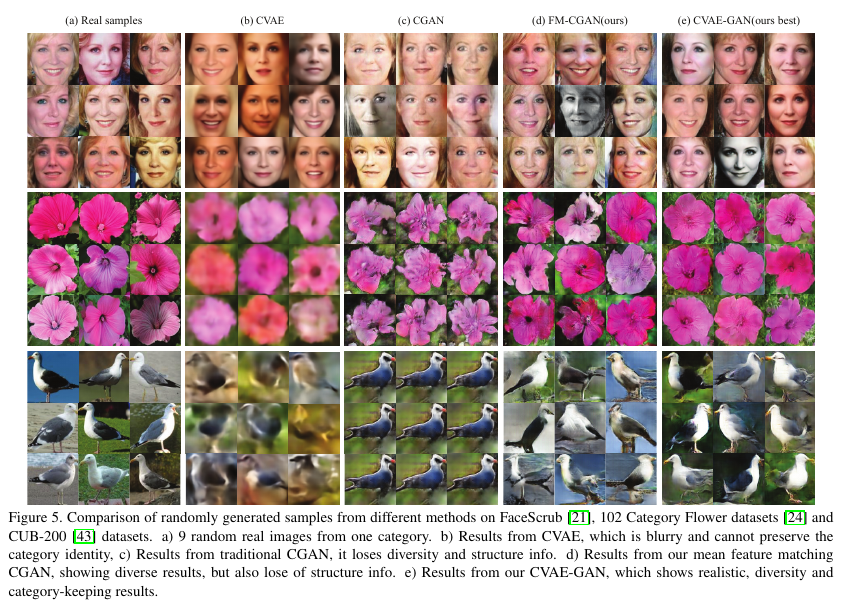
\includegraphics[width=\linewidth,height=0.48\textheight,keepaspectratio]{assets/comparison.png}
    \source{Paper Figure 5: real samples, CVAE, CGAN, FM-CGAN, and CVAE-GAN.}
    \vspace{0.25em}
    {\footnotesize CVAE-GAN retains category identity and within-class diversity more consistently than the baselines shown.}
  \end{column}
  \begin{column}{0.43\textwidth}
    {\small\bfseries Original quantitative results}\par\vspace{0.25em}
    \centering
    \resizebox{\linewidth}{!}{%
    \begin{tabular}{lrr}
      \toprule
      Method & Top-1 acc. & Realism \\
      \midrule
      Real data & 99.61\% & 20.85 \\
      CVAE & 8.09\% & 10.29 \\
      CGAN & 61.97\% & 15.79 \\
      FM-CGAN & 79.76\% & \textbf{19.40} \\
      CVAE-GAN & \textbf{97.78\%} & 19.03 \\
      \bottomrule
    \end{tabular}}
    \vspace{0.75em}
    \raggedright
    {\small\bfseries Original vs. reproduced}\par\vspace{0.2em}
    {\footnotesize
    \textbf{Original evaluation:} 53k generated faces.\par
    \textbf{Smoke reproduction:} training and sampling passed.\par
    \textbf{Paper-scale metrics:} \pending; not comparable yet.\par}
    \source{Metrics reproduced from paper Table 1. ``Realism'' is the paper's Inception Score variant.}
  \end{column}
\end{columns}
\end{frame}

% Slide 5
\begin{frame}{Conclusion and learning}
\begin{columns}[T,onlytextwidth]
  \begin{column}{0.56\textwidth}
    \footnotesize
    \begin{itemize}\setlength\itemsep{0.27em}
      \item \textbf{Reproduction status:} implementation and end-to-end smoke validation succeeded; dataset-scale training and metric replication remain \pending.
      \item \textbf{Major finding:} feature matching stabilizes conditional GAN training, while the encoder and pairwise losses protect diversity and class structure.
      \item \textbf{Reported impact:} synthetic identity augmentation improved LFW verification from 91.87\% to 92.98\% in the paper.
      \item \textbf{Challenges:} legacy Torch code, three datasets with different preprocessing, four-network optimization, and evaluation with a separate classifier.
      \item \textbf{Next improvements:} implement in PyTorch, record seeds and checkpoints, compare FID/KID alongside the legacy score, and run ablations for each loss term.
      \item \textbf{Takeaway:} CVAE-GAN ties each latent code to a real example and trains the generator with feature statistics instead of the discriminator's cross-entropy alone.
    \end{itemize}
  \end{column}
  \begin{column}{0.41\textwidth}
    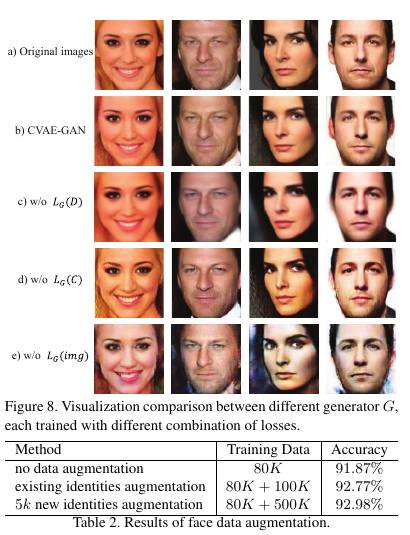
\includegraphics[width=\linewidth,height=0.69\textheight,keepaspectratio]{assets/applications.png}
    \source{Paper Figures 7--8 and Table 2: inpainting, loss ablations, and face augmentation.}
  \end{column}
\end{columns}
\end{frame}

\end{document}
